\begin{frame}
\frametitle{Real data}
\begin{columns}[c]
\column{0.5\textwidth}
Used 550 T1w brain MRI from IXI ({\bf I}nformation e{\bf X}traction from {\bf I}mages) dataset.

\url{http://www.brain-development.org/}

Data from three different hospitals in London:
\begin{itemize}
\item{Hammersmith Hospital using a Philips 3T system}
\item{Guy's Hospital using a Philips 1.5T system}
\item{Institute of Psychiatry using a GE 1.5T system}
\end{itemize}

\column{0.5\textwidth}
\includegraphics[width=0.9\textwidth]{orig_ixi}
\end{columns}
\end{frame}

\begin{frame}
\frametitle{Grey and White Matter}
\begin{columns}[c]
\column{0.26\textwidth}
Segmented into GM and WM.

Approximately aligned via rigid-body.
\column{0.75\textwidth}
\includegraphics[width=0.5\textwidth]{gm_ixi}
\includegraphics[width=0.5\textwidth]{wm_ixi}
\end{columns}

\begin{tiny}
Ashburner, J \& Friston, KJ. \emph{Unified segmentation}. NeuroImage 26(3):839--851 (2005).

\end{tiny}
\end{frame}

\begin{frame}
\frametitle{Diffeomorphic Alignment}
All GM and WM were diffeomorphically aligned to their common average-shaped template.
\begin{center}
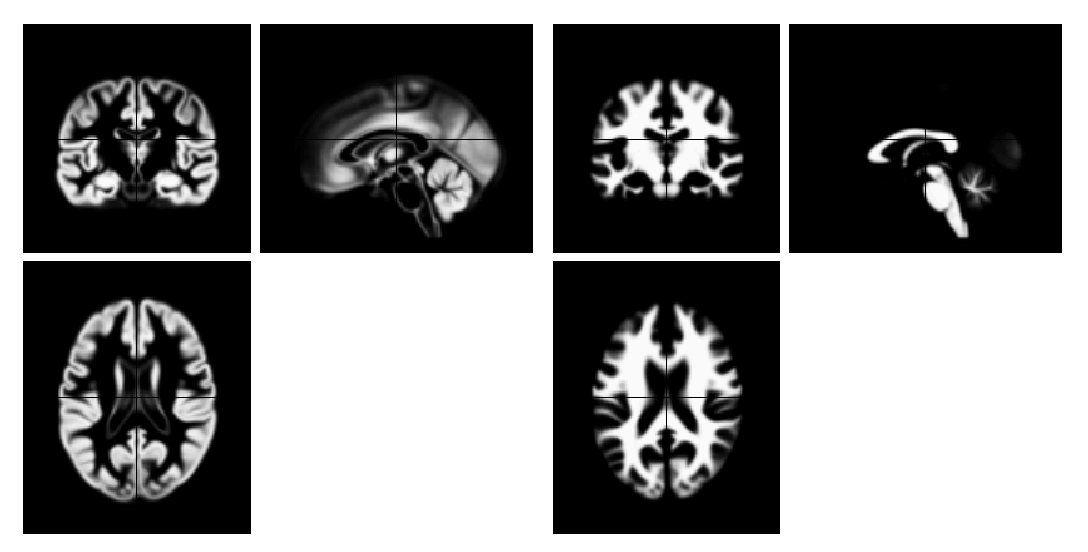
\includegraphics[width=.8\textwidth]{template}
\end{center}

\begin{tiny}
Ashburner, J \& Friston, KJ. \emph{Diffeomorphic registration using geodesic shooting and Gauss-Newton optimisation}. NeuroImage 55(3):954--967 (2011).

Ashburner, J \& Friston, KJ. \emph{Computing average shaped tissue probability templates}. NeuroImage 45(2):333--341 (2009).

\end{tiny}
\end{frame}

